\chapter{Speichersysteme in Videospielen}\label{ch:videospiele}
Anschauen, wie Videospiele Daten speichern und laden\dots
%--------------------------------------------------------------------------


%--------------------------------------------------------------------------
\section{Minecraft}
Minecraft ist ein Sandbox-Spiel\footnote{Ein Sandbox-Spiel lässt Spieler frei entscheiden, was mit der Spielwelt gemacht werden soll. Es gibt keine feste Geschichte im Spiel, die verfolgt werden muss.\cite{ocio2009multi}}, welches von Mojang Studio entwwickelt wurde. Minecraft gilt unter den meistverkauften Videospiele aller Zeiten und kann auf eine Vielzahl von Plattformen gespielt werden.\cite{ignBestSellingVideo} Es wird in einer dreidimensionalen Welt, die aus Blöcken besteht, gespielt und es kann mit Entitäten interagiert werden. Es gibt verschiedene Spielmodi, wie zum Beispiel ein Überlebens- und Kreativmodus. Beim Überlebensmodus geht es hauptsächlich um das Überleben in der Spielwelt, jedoch kann der Spieler frei entscheiden, was er in der Spielwelt machen wird.\cite{minecraftWikiHome}
\todo{Jahr}

In diesem Abschnitt dieser Arbeit wird das Speicher- und Ladesystem von Minecraft genauer betrachtet. Als erstes wird ausgearbeitet, aus welchen Spielobjekten die Welt in Minecraft besteht, um herauszufinden, welche verschiedenen Daten gespeichert werden müssen. Danach wird geschaut, wie diese Daten bei Minecraft aufgeteilt werden, damit nur mit einer Teilmenge der ganzen Daten gearbeitet werden muss. Anschließend wird die Ordnerstruktur einer Spielwelt angeschaut, um ein tieferes Verständnis für die Aufteilung der Daten zu sichern. Danach werden die Formate der Dateien genauer betrachtet, um zu verstehen, wie die einzelnen Daten letztendlich in den Speicher geschrieben werden. Zum Schluss wird angeschaut, wie der Ablauf des gesamten Speicherprozess ist. Es wird erklärt, zu welchen Zeitpunkten der Spielzustand gesichert wird, damit möglichst wenig Daten der Spielwelt verloren gehen. 

\todo{Quelle mit Email}
%\url{https://github.com/Hexeption/MCP-Reborn/tree/1.16}



\subsection{Daten}
Bevor sich das Speicher- und Ladesystem von Minecraft genauer angeschaut werden kann, ist es erstmal wichtig zu wissen, mit welchen Arten von Daten Minecraft arbeitet. Die Spielwelt in Minecraft besteht aus verschiedenen Blöcken, Entitäten\todo{Entitäten vs Entitys} und Items. 

\textit{Blöcke} werden in Minecraft nicht einzeln behandelt, sondern als Section, ein Bereich von 16x16x16-Block, gespeichert. Mehr zu dieser Aufteilung bei Minecraft gibt es im Abschnitt \ref{ssec:datenaufteilung}. Informationen, die zu so einem Block gehören, sind die Position, BlockID, Block Zustände und Informationen zum Licht. Die Position eines Blocks wird in der Reihenfolge y-, z- und x-Koordinate gespeichert, für bessere Komprimierung. Jeder Blocktyp hat eine eigene BlockID, die diesen Block genau identifiziert. Der Zustand eines Blocks wird für jede Section in einer Liste namens "BlockStates" abgespeichert. Informationen dessen Zustands können zum Beispiel sein, in welcher Himmelsrichtung der Block plaziert wurde, welche Rotation der Block hat und ob der Block am brennen ist. Welche Zustände ein Block haben kann, hängt auch von dem Blocktyp ab.\cite{minecraftBlockStates} Bei den Informationen zum Licht jedes Blocks gibt es für jede Section zwei Listen namens "BlockLight" und "SkyLight". "BlockLight" speichert wieviel Licht jeder Block ausstrahlt und "SkyLight" wieviel jeder Block an Licht abbekommt. Zusätlich gibt es noch sogenannte Block Entitys, die aber nichts mit den Entitäten des Spieles zu tun haben. Diese Speichern zusätliche Informationen zu einem Block, die in der "BlockStates"-Liste nicht gespeichert werden konnten.\cite{minecraftChunkFormat}
%Weitere Quelle: ChunkSerializer.java:write()

Eine Entität kann ein Spieler, ein Tier oder Monster sein. Die wichtigste Information einer Entität ist die Position, Geschwindigkeit und Rotation dieser. Des weiteren gibt es viele weitere Informationen zu einer Entität, wie die Luft die die Entität noch übrig hat zum Überleben, die Distanz die eine Entität schon gefallen ist oder wie lange eine Entität noch brennen wird.\cite{minecraftEntityFormat}
%Weitere Quelle: Entity.java:writeWithoutTypeID()

\textit{Items} bei Minecraft existieren im Inventar, in Kisten, in Item Frames oder in Armor Stands\todo{Englisch}. Wenn ein Spieler ein Item fallen lässt, dann werden diese als Entitäten in die Welt platziert und als solche gespeichert. Manche Items können in die Welt platziert werden und werden dann zu neuen Blöcken oder Entitäten. Jedes Item hat die Information "Count", "Slot", "id" und "tag". "Count" und "Slot" definieren, wieviele Items in welchem Inventarplatz liegen. Jedes Item hat dabei eine eigene Identifikationsnummer, mit der diese gespeichert werden. "tag" gibt noch zusätliche Informationen über ein Item, wie die Haltbarkeit oder ob ein Item unzerbrechlich ist.
\cite{minecraftPlayerdatFormat}
\cite{minecraftItem}

%Item werdeb z.B. in player.dat gespeichert



\subsection{Datenaufteilung} \label{ssec:datenaufteilung}
Die Spielwelt von Minecraft, mit seinen Blöcken, Entitäten und Items, werden nach einem Chunk-basiertem System aufgeteilt. Dieses System unterteilt die Welt in verschiedene Gruppierungen und Untergruppen, wobei die oberste Ebene die "Welt" selbst ist. In Minecraft bezeichnet eine "Welt" die Spielwelt, die von einem Spieler erstellt werden kann, und diese Welt wird wiederum in die drei Dimensionen "Overworld", "Nether" und "End" unterteilt.\cite{minecraftWorld}

Jede Dimension bekommt seine eigenen Dateien zum Speichern der Daten (siehe \ref{ssec:ordnerstruktur}). Eine Dimension kann theoretisch aus unendlich vielen Blöcken, Entitäten und Items bestehen. Sie wird dabei auf mehrere Regionen aufgeteilt. Eine Region besteht aus 1024 Chunks, wobei sie 32 Chunks breit und 32 Chunks lang ist.\cite{minecraftRegionFile} 

Was die Größe eines Chunks betrifft, so ist sie statisch und beträgt 16 Blöcke in der Länge, 16 Blöcke in der Breite und die Höhe variiert je nach der jeweiligen Höhe der Welt. Seit der Einführung der Minecraft Version 1.18 beträgt die maximale Höhe der Spielwelt 384 Blöcke.\cite{minecraftNewestJavaEdition}\cite{minecraftNewestBedrockEdition} Um diese Struktur weiter zu verfeinern, wird jeder Chunk in Sektionen unterteilt. Eine Sektion besteht aus insgesamt 4096 Blöcken, was bedeutet, dass sie 16 Blöcke in der Länge, Breite und Höhe umfasst.\cite{minecraftChunk}

%Chunk.java:sections



\subsection{Ordnerstruktur} \label{ssec:ordnerstruktur}
Ein Spieler kann in Minecraft verschiedene Spielwelten erstellen. Dabei bekommt jede dieser Spielwelten einen eigenen Ordner. Wie so ein Ordner aufgebaut ist, ist in der Ordnerstruktur aus \ref{lst:ordnerStrukturMinecraft} zu sehen. Die nicht-markierten Knoten entsprechen einem Ordner und die blauen Knoten sind Dateien in dem Speichersystem. In dem Ordner einer Welt sind noch ein paar weitere Ordner und Dateien, diese sind aber nicht relevant für diese Arbeit. Die erste Datei in dem Ordner, die "level.dat"-Datei, speichert globale Daten über die Spielwelt ab. In den Ordnern "playerdata", "stats" und "advancements" werden Spielerinformationen abgespeichert, über eine "<uuid>.dat"- oder "<uuid>.json"-Datei. Die "uuid" wird dabei durch die Identifikationsnummer des Spielers ersetzt. Wenn alleine gespielt wird, werden viele Spielerdaten auch in der "level.dat"-Datei gespeichert. In dem "stats"- und "advancements"-Ordner werden Statistiken und Fortschritte von jedem Spieler der Welt gespeichert. Falls eine Welt im Mehrspielermodus gespielt wird, enthalten die Dateien im "playerdata"-Ordner alle restlichen Informationen eines Spielers.\cite{minecraftPlayerdatFormat}. Die restlichen Ordner und Dateien speichern den Zustand der Spielwelt. Bei Minecraft gibt es zum Beispiel Weltkarten, die Teile der Spielwelt anzeigen können. Jede Weltkarte kann dabei unterschiedliche bereiche der Welt anzeigen, deshalb gibt es für jede Weltkarte eine "map\_<\#>.dat"-Datei, die den Zustand einer Weltkarte speichert. Die "villages.dat"-Datei speichert die Zustände aller Dörfer der Spielwelt, denn jedes Dorf ist ein komplexes System aus verschiedenen zufällig generierten Entitäten und Gebäuden. Da die Spielwelt von Minecraft aus verschiedenen Dimensionen, namens "Overworld", "Nether" und "End" besteht, werden manche Daten auf verschiedenen Ordnern verteilt. Im "DIM-1"-Ordner werden Informationen zu der "Nether"-Dimension gespeichert und der "DIM1"-Ordner ist für die "End"-Dimension. Die "entities"- und "region"-Ordner zum Beispiel enthalten Informationen über die Entitäten und Regionen der Spielwelt und sind auch in den Ordnern der verschiedenen Dimensionen zu finden. Alle Entitäten und Regionen, die in keinem "DIM-1"- oder "DIM1"-Ordner gespeichert wurden, gehören zu der "Overworld"-Dimension.\cite{minecraftFolderStruc}

\begin{listing}[htp]
    \dirtree{%
    .1 world.
        .2 \textcolor{blue}{level.dat}.
        .2 playerdata.
            .3 \textcolor{blue}{<uuid>.dat}.
        .2 stats.
            .3 \textcolor{blue}{<uuid>.json}.
        .2 advancements.
            .3 \textcolor{blue}{<uuid>.json}.
        .2 data.
            .3 \textcolor{blue}{idcounts.dat}.
            .3 \textcolor{blue}{map\_<\#>.dat}.
            .3 \textcolor{blue}{villages.dat}.
            .3 \dots.
        .2 entities.
        .2 region. 
            .3 \textcolor{blue}{r.<\#>.<\#>.mca}.
        .2 DIM-1.
            .3 entities.
            .3 region.
                .4 \textcolor{blue}{r.<\#>.<\#>.mca}.
            .3 \dots.
        .2 DIM1.
            .3 entities.
            .3 region.
                .4 \textcolor{blue}{r.<\#>.<\#>.mca}.
            .3 \dots.
        .2 \dots.
    } 
    \caption{Ordnerstruktur einer Spielwelt in Minecraft\cite{minecraftFolderStruc}}
    \label{lst:ordnerStrukturMinecraft}
\end{listing}



\subsection{Speicherformate}
Wie schon im vorherigen Abschnitt zu sehen ist, besitzt Minecraft eine handvoll verschiedener Formate, zum Speichern der Daten. Die Dateien haben Formate wie "dat", "mca" und "json". Natürlich existieren auch noch weitere Formate, wie PNG-Dateien für Texturen, da diese Dateien zu den statischen Daten dazugehören, werden diese nicht weiter betrachtet.   

Das DAT-Format wird für jegliche Arten von Informationen verwendet, sei es Video, Audio, PDF oder jede andere Art von Daten. Ein Programm kann DAT-Dateien erstellen und spezifisch für dieses Programm Daten abspeichern und lesen. Für andere Programme sind diese Daten nicht sonderlich hilfreich, da sie für ein spezifisches Programm erstellt wurden.\cite{adobeWhatDAT} Dieses Format wird zum Beispiel für die globalen Spielwelt Informationen in der "level.dat"-Datei oder für Spielerdaten in "<player>.dat"-Dateien, falls die Spielwelt auf einem Server gehosted wird (siehe \ref{ssec:ordnerstruktur}).\cite{minecraftPlayerdatFormat}\cite{minecraftFolderStruc}. 
Die Daten werden dabei im eigenen Format namens Named Binary Tag (NBT)\todo{Abkürzungsverzeichnis} in diese Dateien geschrieben. Diese Format ist ähnlich zu dem JSON-Format, denn die Daten werden auch hier im Schlüssel-Wert-Prinzip behandelt. Das NBT-Format bietet eine Vielzahl an Datentypen, wie Byte, Boolean, verschiedene Zahlen Datentypen, String, List, Compound und Array. Der List-Datentyp ist zum Speichern von mehreren Werten, ohne Schlüssel. Compound ist eine geordnete Liste von Schlüssel-Wert-Paaren. Nachträglich werden in den meisten Fällen die NBT-Dateien mit GZip komprimiert.
\cite{minecraftNBT}

Minecraft Anvil (MCA)\todo{Abkürzungsverzeichnis} ist ein Dateiformat, zum Speichern von Chunk-Daten. Dabei wird in einer Datei eine Region, also eine Gebiet aus 32x32 Chunks, gespeichert. Jede Datei bekommt dann den Namen "r.<x>.<z>.mca", wobei x und z mit den x und z Koordinaten der Region ersetzt wird. Falls die Koordinaten einer Region gesucht werden, in der ein Chunk drin ist, müssen die Chunk-Koordinaten durch 32 geteilt und abgerundet werden. Eine MCA-Datei fängt mit einem 8 KiB Header an, der in zwei 4 KiB Blöcken unterteilt ist. Der erste Block beschreibt die Position der Chunks in der Region und der zweite Block speichert die Zeit, wann jeder Chunk zuletzt aktualisiert wurde. Nach dem Header werden alle Zustände der Chunks einer Region gespeichert. Dabei wird für jeden Chunk erst die Länge der Daten in Bytes angegeben, dann die Art der Komprimierung und anschließend die komprimierten Daten.\cite{minecraftRegionFile}\cite{minecraftAnvilFile} Auch in diesen Dateien werden die Daten im NBT-Format in komprimiert Form gespeichert.\cite{minecraftNBT}

Das JSON-Format wird für das Speichern von Texten und kleineren Daten verwendet. In Minecraft gibt es Bücher, Schilder und Labels, die der Spieler beschriften und mit Text füllen kann. Bücher zum Beispiel werden dann zwar im NBT-Format in den Dateien zu den Spielerdaten gespeichert, aber die Seiten der Bücher werden als serialisierten JSON-Text gespeichert.\cite{minecraftPlayerdatFormat} Die "advancements"- und "stats"-Ordner, die im Abschnitt \ref{ssec:ordnerstruktur} vorgestellt wurden, speichern die Fortschritte der einzelnen Spieler auch im JSON-Format ab. Ansonsten wird JSON hauptsächlich für statische Daten, wie das Verhalten von Entitäten, Blöcken und Items oder Anleitungen für das Bauen von Spielgegenständen.\cite{minecraftJSON}

%Siehe auch: RegionFileCache.java:loadFile(), SaveFormat.java:convertRegions()

\subsection{Speichervorgänge}
In den vorherigen Abschnitten wurde detailliert erörtert, welche Daten in Minecraft gespeichert werden und in welcher Form dies geschieht. Nun stellt sich die Frage nach dem genauen Ablauf des gesamten Speicherprozesses und den Zeitpunkten, zu denen die Daten gesichert werden.

Der Spielzustand einer Welt in Minecraft wird zu verschiedenen Zeitpunkten im Spielverlauf gesichert. Zunächst wird der initiale Zustand der Spielwelt gespeichert, wenn eine Welt neu generiert wird. Doch darüber hinaus erfolgen während das Spiel gespielt wird sowohl automatische als auch manuelle Speicherprozesse.\cite{minecraftSpielstandSpeicherung}

Manuelle Speicherungen finden statt, wenn der Spieler die Pause-Taste betätigt, die in Minecraft der "Esc"-Taste entspricht. Damit hat der Spieler die Möglichkeit, den aktuellen Zustand seiner Welt bewusst zu sichern.\cite{minecraftSpielstandSpeicherung} 

Automatische Speicherungen erfolgen hingegen in regelmäßigen Intervallen. Der Spielzustand wird alle fünf Minuten automatisch gesichert, um sicherzustellen, dass selbst bei unvorhergesehenen Ereignissen oder einem möglichen Absturz des Spiels nur minimaler Fortschritt verloren geht.\cite{minecraftSpielstandSpeicherung}

Chunks die zu weit weg von dem Spieler sind, werden bei Minecraft entladen, da es sehr viele Ressourcen brauchen würde, alle Chunks geladen zu lassen, auch wenn sie nicht aktiv verwendet werden. Bevor diese entladen werden, wird der Zustand des Chunks automatisch gesichert. Dies gewährleistet, dass keine relevanten Chunk-Informationen verloren gehen und diese bei Bedarf wiederhergestellt werden können.\cite{minecraftSpielstandSpeicherung}

Insgesamt sorgen diese verschiedenen Speichermechanismen in Minecraft dafür, dass der Spielverlauf zuverlässig und in verschiedenen Situationen gesichert wird, um den Verlust von Fortschritt auf ein Minimum zu reduzieren.

%Siehe auch: Minecraft.java:createWorld()
%Siehe auch: IntegratedServer.java:tick()



\subsection{Ladevorgänge}



\subsection{Fazit}
\begin{itemize}
    \item Chunk System mit fester Größe, da Limit an Elementen pro Chunk?
\end{itemize}

\todo{Irgendwie zusammenfassen, welche Strategien Minecraft verwendet?}
%--------------------------------------------------------------------------



%--------------------------------------------------------------------------
\section{Factorio}
Factorio ist ein Spiel, wo das Hauptziel ist, eine Fabrik aufzubauen. Als Spieler muss man sich um Ressourcen kümmern, die abgebaut werden müssen, um damit neue Technologien zu erforschen und eine Infrastruktur aufzubauen. Um eine möglichst große Ausbeute für die eigene Fabrik zu erreichen, kann die Produktion automatisiert werden. Im Spiel gibt es außerdem noch Einheimische, die die Ausbeutung der Ressourcen anhalten wollen. Deshalb muss der Spieler zusätzlich zu dem Aufbauen seiner Fabrik diese auch noch vor den Einheimischen verteidigen, damit sie nicht kaputt geht. Factorio wurde in C++ geschrieben und 2016 auf der Plattform "Steam" veröffentlicht. Mittlerweile kann Factorio auf Windows, macOS, Linux und der Nintendo Switch gespielt werden.\cite{factorioMain}\cite{factorioPressFactorio}

% Allgemein benutzt Factorio ein "Deterministic save load"
% \url{https://gist.github.com/Rseding91/a309cf0a30782a2e96ef081c39326f42}

Offizielle Wiki: \url{https://wiki.factorio.com/}\cite{factorioPressFactorio}\todo{Quelle Email und Wiki}

\subsection{Daten}
Factorio benutzt Serialisierung und Deserialisierung, verwendet dabei aber verschiedene Formate zum Speichern der Daten. Welche verschiedenen Arten von Daten dann das Spiel hat, zeigt die Abbildung \ref{fig:factorioSaveStatistic}. Das Kreisdiagramm zeigt welche Arten von Daten wie viel Speicherplatz benötigen, bei 40 MB unkomprimierten Daten. Ungefähr 70\% des Speicherplatzes verbrauchen drei Kategorien der Spielobjekte, die Dekorations-Objekte, Tiles und Entitäten. Tiles sind Rechtecke, die das kleinste Stück in der Spielwelt darstellen. Die Tiles sind auch die Maßeinheiten für alle Gebiets- und Distanzabmessungen. Die Größe von Entitäten wird auch in Tiles angegeben. Zum Beispiel ist das "Rocket Silo", die größte Entität in dem Spiel, neun Tiles breit und lang. Die Spielwelt hat eine maximale Größe von zwei Millionen Tiles in der Breite und Länge, also vier Trillionen Tiles.\cite{factorioMapStructure} Die restlichen Daten sind aus der Blueprint Bibliothek, Physikalische Kräfte, Transportbänder, Oberfläche und Chunk Daten und weiteren kleineren Daten.\cite{factorioFridayFacts270} Die Blueprint Bibliothek ist ein virtuelles Inventar, welche Blueprint-artige Items speichert.\cite{factorioBlueprintLibrary} Ein Blueprint ist zum Duplizieren von Fabrikbereichen. Diese können als Blueprint gespeichert und in der Spielwelt dann eingefügt werden.\cite{factorioBlueprint}. Da ein Spieler eine Vielzahl an Blueprints erstellen kann, müssen diese beim Speicherprozess mit einbezogen werden. Transportbänder sind wichtig zum maximieren der Produktion und Automatisierung dieser. Sie transportieren die abgebauten oder hergestellten Ressourcen. Was genau in einem Chunk drin ist, ist in dem Abschnitt \ref{ssec:factorioDatenaufteilung} zu sehen. 

\begin{figure}[htp]
    \centering
    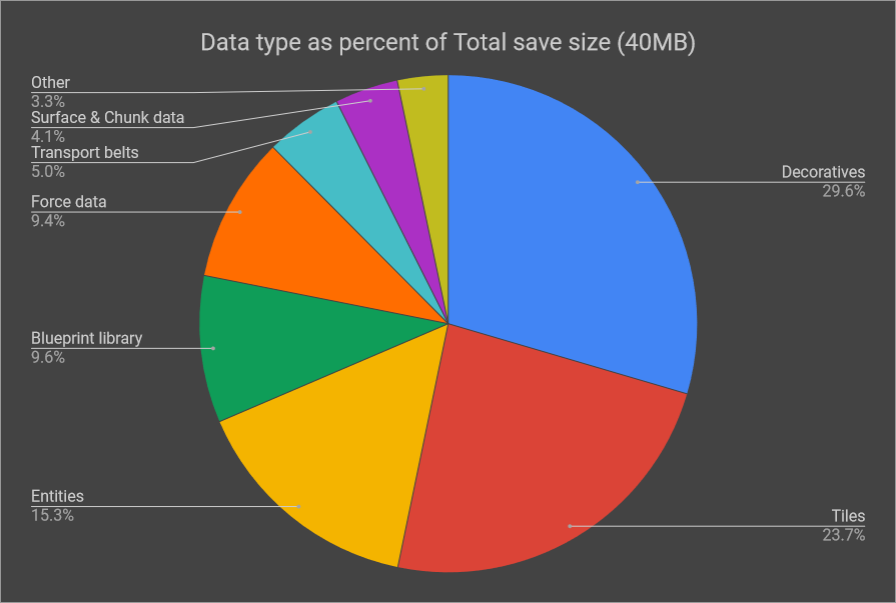
\includegraphics[width=0.9\textwidth]{images/factorio_save_statistic.png}
    \caption{Anteil der Datentypen beim Speichern\cite{factorioFridayFacts270}}
    \label{fig:factorioSaveStatistic}
\end{figure}



\subsection{Datenaufteilung} \label{ssec:factorioDatenaufteilung}
Chunks (32x32 Tiles) \cite{factorioMapStructure}



\subsection{Ordnerstruktur}
User data Ordner:
\begin{itemize}
    \item ./saves (Save files)
    \item ./mods (Mods)
    \item ./script-output (Script-output, z.B. von Spiel Screenshots)
    \item ./scenarios (Lokale Szenarien)
    \item ./config/config.ini (Lokale Einstellung)
    \item factorio-*.log (Log files)
    \item factorio-dump-*.dmp (Crash dump files)
\end{itemize}

%2.8.2023
\url{https://wiki.factorio.com/Application_directory} %Offizielle Factorio Wiki laut Seite



\subsection{Speicherformate}
\url{https://wiki.factorio.com/index.php?title=Achievement_file_format&oldid=179094}\\
\url{https://wiki.factorio.com/index.php?title=Blueprint_string_format&oldid=190672}\\
\url{https://wiki.factorio.com/index.php?title=Map_exchange_string_format&oldid=187695}\\



\subsection{Speichervorgänge}
Kurzgefasst:
\begin{enumerate}
    \item ID Mapping speichern (\url{https://www.factorio.com/blog/post/fff-259}) %2.8.2023
    \item Map Daten speichern
\end{enumerate}

Detaillierter:
\begin{enumerate}
    \item Volles leeren der Garbage Collection von allen Lua Zuständen
    \item Löschen von temporären Map Daten, die während des Speicherprozesses entstanden sind
    \item ID mapping speichern (ID mapping für alles was IDs benutzt)
    \item Speichern der Prototypenmigrationen
    \item Rest, der gespeichert weden soll, abspeichern
    \item SaveHelpers speichern
\end{enumerate}
%2.8.2023
\url{https://gist.github.com/Rseding91/a309cf0a30782a2e96ef081c39326f42} 

\subsection{Ladevorgänge}
Kurzgefasst:
\begin{enumerate}
    \item Map Version überprüfen
    \item Überprüfen ob Mods hinzugefügt/gelöscht/verändert wurden
    \item invalide/korrupte save files finden 
\end{enumerate}

Detaillierter:
\begin{enumerate}
    \item Map-Version überprüfen (save file map und die map in der die save file map geladen wird)
    \item Überprüfen, ob aktive Mods oder die Mod-Einstellungen sich verändert haben (wenn ja, müssen Aktionen nach dem laden durchgeführt werden) und setze flag wenn das der Fall ist
    \item ID mapping laden
    \item Angewandte Migrationen laden und nicht angewandte Migrationen ausführen
    \item Standard Map Daten laden (Enitäten, Chunks, Forces, Züge)
    \item load in allen LoadHelpers aufrufen
    \item Inszenierte (???) Veränderungen ausführen
    \item Enitäten, die Ladeprobleme hatten, nachladen
    \item Targeters wiederherstellen
    \item setup bei allen LoadHelpers ausrufen
    \item Wenn Prototyp Daten verändert wurden Elektrisches Netz Daten clearen
    \item setup aller transport belt connectible Entitäten aufrufen
    \item Ruf setup von Entität auf, wenn diese während Laden erstellt wurde und nicht existierte, als die Map zuletzt gespeichert wurde
    \item postLoadHook für die Map aufrufen
    \item Tile Probleme fixen, nachdem alle Enitäten geladen wurden und setup fertig ist
    \item Ruf bei allen PreFinalLoadHelper setup auf
    \item Ruf bei allen FinalLoadHelper setup auf
    \item Für alle Oberflächen postSetup aufrufen
    \item Lua Daten laden und wiederherstellen
    \item "configuration changed" Lua event ausführen
\end{enumerate}
%--------------------------------------------------------------------------

%--------------------------------------------------------------------------
\section{Terraria}

In \url{https://store.steampowered.com/news/app/105600/view/4560463273436543493} steht die neue offizielle Doku Seite für Terraria (\url{https://terraria.wiki.gg/wiki/Terraria_Wiki})


\subsection{Daten}
Welche Klassen gibt es bei Terraria (Blöcke, Chunks,...) und welche Daten 
beinhalten diese.

\subsection{Ordnerstruktur}

\subsection{Speicherformate}
World-Dateien, Player-Dateien, Konfigurationsdateien 

\subsection{Datenaufteilung}
Kein Chunksystem, alles in einer Datei gespeichert. Aber Inventar, Position
usw. werden in verschiedenen Daten gespeichert.

\subsection{Speichervorgänge}

\subsection{Ladevorgänge} 
%--------------------------------------------------------------------------


\iffalse
%--------------------------------------------------------------------------
\section{Ein Spiel}
Beschreibung von dem Spiel

\subsection{Daten}
Welche Klassen gibt es bei <Spielname> (Blöcke, Chunks,...) und welche Daten 
beinhalten diese.

\subsection{Ordnerstruktur}

\subsection{Speicherformate}

\subsection{Datenaufteilung}

\subsection{Speichervorgänge}

\subsection{Ladevorgänge}
\fi
